\documentclass[./../../paper.tex]{subfiles}
\graphicspath{{\subfix{./../../figures/}}}

\begin{document}
Having discussed the previous work on counterfactual sequence generation, a couple of challenges emerge.
First, we need to generate on a set of criteria and therefore, require complex loss and evaluation metrics, that may or may not be differentiable. Second, they cannot to be logically impossible, given the dataset.
Hence, we have to restrict the space to counterfactuals of viable solutions, while being flexible enough to not just copy existing data instances.
Third, using domain knowledge of the process significantly reduces the practicality of any solution. Therefore, we have to develop an approach, which requires only the given log as input while not relying on process specific domain knowledge. This begs the question, whether there is a method to generate sequential counterfactuals that are viable, without relying on process specific domain knowledge. In terms of specific research questions we try to answer:

\begin{itemize}
    \item[RQ:] How do we generate counterfactual sequences while incorporating structural differences between the factual sequence and the counterfactual sequence?
          \begin{itemize}
            \item[RQ1:] How can we employ existing methods to compute viability so that its optimization incorporates information about the structure of the sequence?
              \item[RQ2:] To what extent can we generate counterfactuals that fulfill the criteria to be viable?
              \item[RQ3:] How does an algorithm, which optimizes multiple viability quality metrics, perform against other approaches?
          \end{itemize}
\end{itemize}

\noindent We approach these questions, by proposing a schematic framework which allows the exploration of several independent components. \autoref{fig:framework-simplified} shows the conceptual framework of the base approach visually.

\begin{figure}[htb]
    \centering
    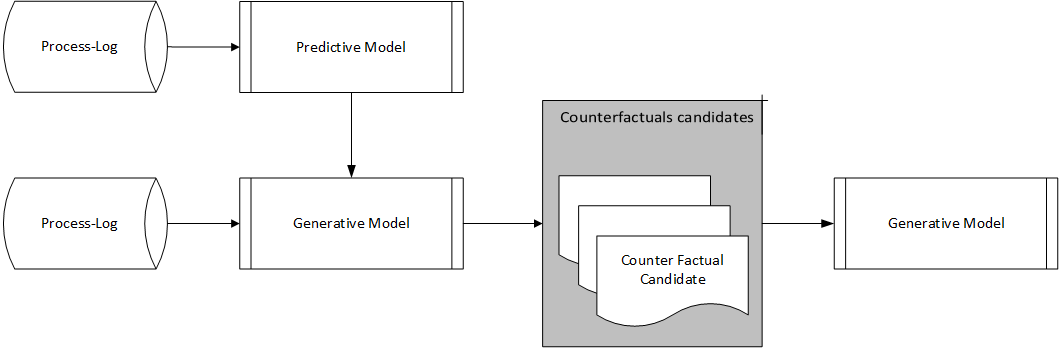
\includegraphics[width=0.9\textwidth]{figures/framework_simplified.png}
    \caption{A simplified schematic representation of the framework which is explored in this thesis.}
    \label{fig:framework-simplified}
\end{figure}

\noindent The framework contains three parts. First, we need a pre-trained predictive component, which we aspire to explain. The component should \emph{accurately} predict the outcome of a process at any step. The accuracy-condition is favorable, but not necessary. If the component is accurately modelling the real world, we can draw real-world conclusions from the explanations generated. If the component is inaccurate, the counterfactuals only explain the prediction decisions and not the real world. The second part requires a generative component. The generative component needs to generate viable sequential counterfactuals which are logically \emph{plausible}. A plausible counterfactual is one whose outcome can be  predicted by the predictive component. If the predictive component cannot predict the counterfactual sequence, we can assume that the generative model is \emph{unfaithful} to the predictive component that we want to explain. The third component is the evaluation metric upon which we decide the viability of the counterfactual candidates.

% TODO: Think of whether we have to include it.
% \optional{This part is not fully thought out.}
For the evaluation, we have to show the following:
\begin{itemize}
    \item[RQ2-H1:] If we use a viability function which incorporates multiple criteria to determine counterfactuals, we consistently retrieve more viable counterfactuals, than choosing the counterfactuals the at random.
    \item[RQ2-H2:] The generated counterfactuals consistently outperform the most viable counterfactuals among examples in the dataset.
    \item[RQ3-H1:] The results of the counterfactual are comparable to other existing literature.
          % \item[RQ2-H1:] The counterfactual generation consistently identifies the most viable counterfactual in the dataset faster than a random search.
\end{itemize}





\end{document}